\chapter{Tools}

\subsection{Big Data}
Big Data is a phrase used to mean a massive volume of both structured and unstructured data that is so large it is difficult to process using traditional database and software techniques. In most enterprise scenarios the volume of data is too big or it moves too fast or it exceeds current processing capacity.

\section{Hadoop}
Hadoop is an open source distributed processing framework that manages data processing and storage for big data applications running in clustered systems.It is at the center of a growing ecosystem of big data technologies that are primarily used to support advanced analytics initiatives, including predictive analytics, data mining and machine learning applications. Hadoop can handle various forms of structured and unstructured data, giving users more flexibility for collecting, processing and analyzing data than relational databases and data warehouses provide.


\subsubsection{Single Node} 
Single node cluster means only one Data Node running and setting up all the Name Node, Data Node, Resource Manager and Node Manager on a single machine. This is used for studying and testing purposes. For example, let us consider a sample data set inside a healthcare industry. So, for testing whether the Oozie jobs have scheduled all the processes like collecting, aggregating, storing and processing the data in a proper sequence, we use single node cluster. It can easily and efficiently test the sequential workflow in a smaller environment as compared to large environments which contains terabytes of data distributed across hundreds of machines. 
\subsubsection{Multi Node} 
While in a Multi node cluster, there are more than one Data Node running and each Data Node is running on different machines. The multi node cluster is practically used in organizations for analyzing Big Data. Considering the above example, in real time when we deal with petabytes of data, it needs to be distributed across hundreds of machines to be processed. Thus, here we use multi node cluster.

\subsection{Pig }
Pig is a high-level programming language useful for analyzing large data sets. A pig was a result of development effort at Yahoo!.
In a Map Reduce framework, programs need to be translated into a series of Map and Reduce stages. However, this is not a programming model which data analysts are familiar with. So, in order to bridge this gap, an abstraction called Pig was built on top of Hadoop.

Apache Pig enables people to focus more on analyzing bulk data sets and to spend less time writing Map-Reduce programs. Similar to Pigs, who eat anything, the Pig programming language is designed to work upon any kind of data. That's why the name, Pig! 

\subsection{Sqoop }
Sqoop is a tool designed to transfer data between Hadoop and relational database servers. It is used to import data from relational databases such as MySQL, Oracle to Hadoop HDFS, and export from Hadoop file system to relational databases.
\subsection{HIVE}
Apache Hive is a data warehouse software project built on top of Apache Hadoop for providing data query and analysis. Hive gives a SQL-like interface to query data stored in various databases and file systems that integrate with Hadoop.
\section{Big Bank, Big Problem}
A leading banking and credit card services provider is trying to use Hadoop
technologies to handle and analyze large amounts of data.\newline
Currently, the organization has data in the RDBMS but wants to use the
Hadoop ecosystem for storage, archival, and analysis of large amounts of
data.
\section{Creating the Hadoop Cluster and Deploying Test Codes}
For any Big Data project, a proper environmental setup is mandatory. In
real world scenarios, a Hadoop cluster can consist of 40K clusters/nodes.
As it is not possible for us to build such a huge setup in an academic lab,
we will be going with minimal 2 node cluster and simulate the ingestion,
cleaning, analysis and send the report to the downstream team.
Create a Pseudo-Distributed Node Cluster and deploy all the test codes
using Maven and SBT.\newpage
\subsection{Data Ingestion}
Bring data from RDBMS to HDFS. This data import must be incremental
and should happen every 2 minutes.
\newline
Following tables have to be imported:
\begin{figure}[H]
\centering
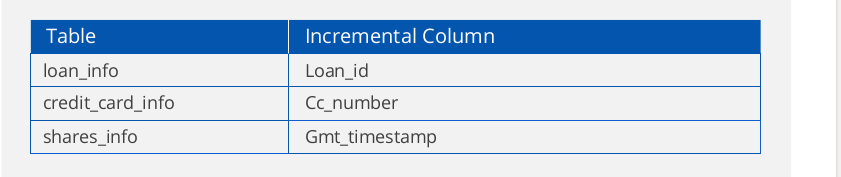
\includegraphics[width=12cm,height=3cm]{dataingestion.png}
    \caption{Data Ingestion}
\end{figure}
\newline
All these data must be encrypted in HDFS. The HDFS data should be
compressed to store less volume.\newline
The Sqoop password must also be encrypted.
\newline
Table Details:
\subsection{Loan\_info}
This table has following columns:\newline
\begin{figure}[H]
\centering
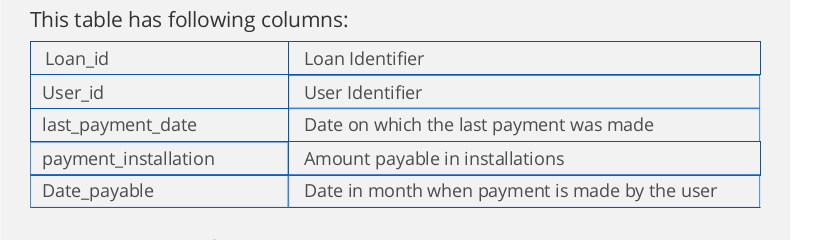
\includegraphics[width=12cm,height=3cm]{loan_info.png}
    \caption{Loan\_info}
\end{figure}\newpage
\subsection{Credit\_card\_info}
This table has the following columns:
\begin{figure}[H]
\centering
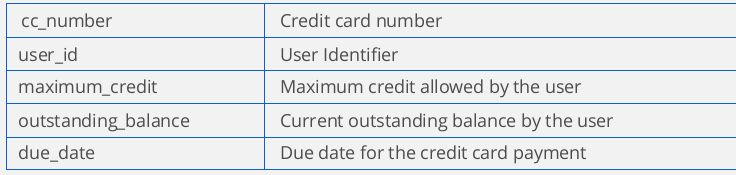
\includegraphics[width=12cm,height=3cm]{creditcard1.png}
    \caption{Credit\_card\_info}
\end{figure}
\newline
\subsection{Shares\_info}
This table has the following information:
\begin{figure}[H]
\centering
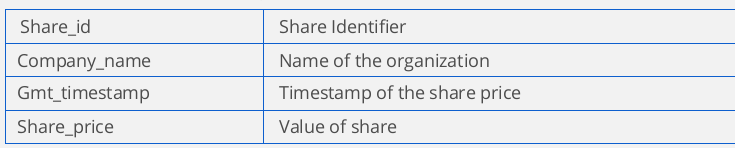
\includegraphics[width=12cm,height=3cm]{sharesinfo1.png}
    \caption{Shares\_info}
\end{figure}
\newline
\subsection{Analysis}
\item Find out the list of users who have at least 2 loan installments pending.
\item Find the list of users who have a healthy credit card but outstanding loan
account.
\items Healthy credit card means no outstanding balance.
\newline For every share and for every date, find the maximum profit one could
have made on the share. Bear in mind that a share purchase must be
before share sell and if share prices fall throughout the day, maximum
possible profit may be negative. \newpage
\subsection{Archival}
The organization has a lot of survey data scattered across different files in
a directory in local file system. Provide a mechanism to effectively store the
small files in Hadoop. It is expected to pack small files together before
actually storing them in HDFS.\newline
Survey files have the following structure:
\begin{figure}[H]
\centering
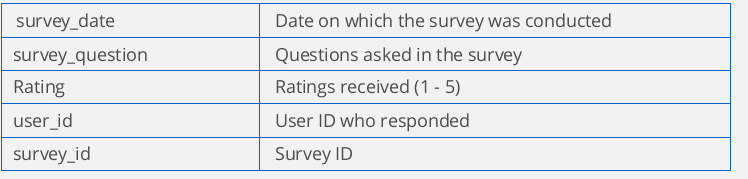
\includegraphics[width=12cm,height=3cm]{surveyfile.png}
    \caption{Survey files}
\end{figure}
\newpage











%The five different levels of the architecture represent the different points of view of
%%\begin{itemize}
% \item \textit{Layer 1}: This level defines the tasks of acquisition, transfer, exchange and
%discovery for the learner as a result of the interactions with his environment. The
%level is seen as two systems exchanging information.
 %\item \textit{Layer 2}: This layer defines the learner’s reaction to the environment. The
%definition is based on the specific design features of learner related modules.
  %\item \textit{Layer 3}: A component system, normalized by IEEE, defines an organization
%of a learning process, seen from the data and control flow point of view.
%  \item \textit{Layer 4}: This level exploits the component %system, directly, in order to
%formalize the technological design constraints. It allows the identification of the
%system’s activities during the learning process. This provides the genric views of
%all the stakeholders and therefore, takes care of their interest.
 % \item \textit{Layer 5}:  \blindtext
%\end{itemize}
%\begin{comment}
%\begin{figure}[htb]
 %\centering
 %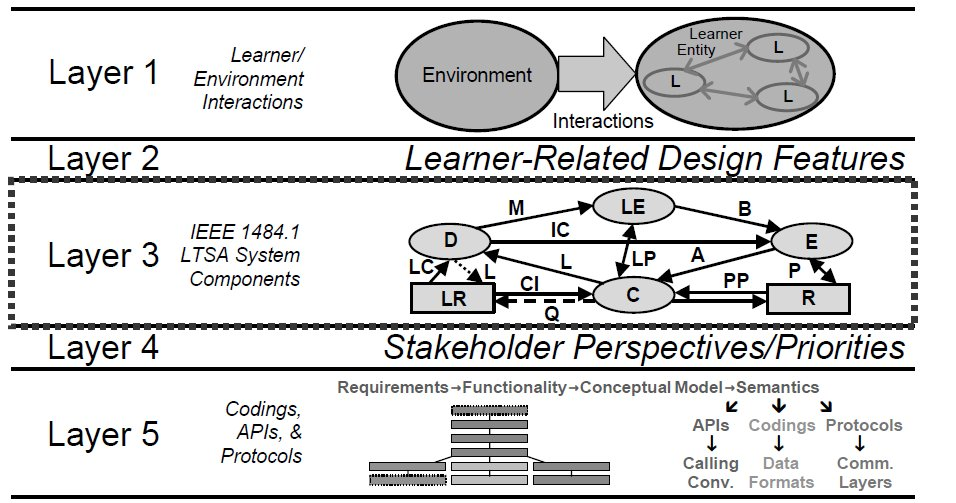
\includegraphics[scale=.4]{m.jpg}
 % m.jpg: 956x503 pixel, 72dpi, 33.73x17.74 cm, bb=0 0 956 503
% \caption{IEEE LTSA Layered Structure\cite{ltsa}}
%\end{figure}
%\end{comment}
%\subsection{A detailed description of LTSA system components at level 3}
% \blindtext types used are \cite{ltsa} (figure.2):
%\begin{enumerate}
 %\item \textit{The interaction context:} This flow of data gives the necessary information for
  %  interpretation of the observations.
%\item \textit{The observations:} This represents the real-time unabridged information concerning the learner activities.
%\item \textit{The acquisition state:} The evaluating process can send or update a learner profile (e.g. a response to a correct answer within a given time).
%\item \textit{The learner profile:} The tutoring process can %consult and modify learner information during the apprenticeship. This is a data-store
   % which updates the learner profile as per data-base management system dictat.
%\item \textit{The evaluation:} It informs the tutoring process of the present state of the
   % learner profile so as to optimize the learning process.
%\begin{comment}
%\begin{figure}[htb]
 %\centering
 %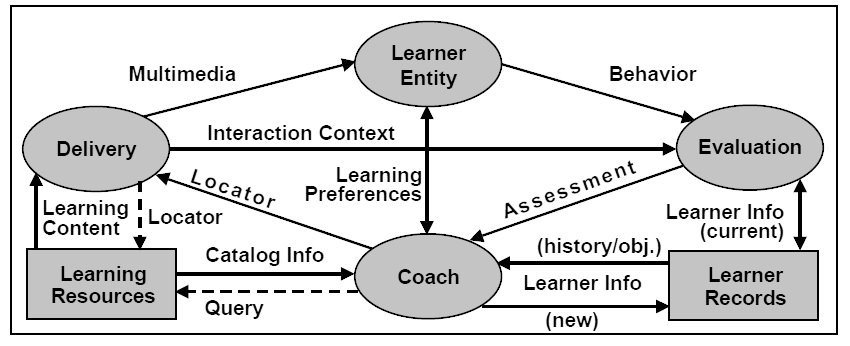
\includegraphics[scale=.6]{rj.jpg}
 % rj.jpg: 850x346 pixel, 72dpi, 29.99x12.21 cm, bb=0 0 850 346
% \caption{IEEE LTSA Layer-3 (System Components)\cite{ltsa}}
%\end{figure}
%\end{comment}
%\item  \textit{The learner preferences:} The tutoring process negotiates the teaching parameters with the learning actor(s).
%\item  \textit{The multimedia data:} This flow of data allows the learning process to use simultaneous pedagogical multimedia resources such as video, audio, text and
   % graphics. All these contents are devloped and designed as per scheme of e-Learning.
%\item  \textit{The locality:} This data or control flow indicates where to find a given pedagogical resource.
%\item  \textit{The pedagogical contents:} This data flow has the coded pedagogical material. The content presentation, in an appropriate format, is an
 %   outcome of this data flow.
%\item  \textit{The catalogued inquiries and information:} The tutoring process can carry out
 %   simple requests to find appropriate learning objects for a course. These requests
  %  may contain search criteria based on the learner’s preferences, the evaluation
   % results and the course information.

%\end{enumerate}  The role and the behavior of the different components are described using a
%learner scenario, which is divided into eight identified scenarios:
%\begin{enumerate}
 %\item The teaching style, the pedagogical choices and the acquisition methods are
%negotiated with the learner.
%\item The learning process is observed and evaluated in a context of action and
%interaction with the system.
%\item The evaluating process gives observations and indications about the learner
%style and/or information about the functioning /the state of the system.
%\item This data is stored in a data bank dedicated to the learner.
%\item The tutoring process analyses the learner’s performance from his assessments,
%his preferences, his past history and his future perspectives.
%\item This same process searches for suitable learning object using resource bank
%requests.
%\item The tutoring process extracts the pedagogical content from the proposed
%resources. It transmits the resource references to the diffusion process, organizing
%them, for example, into a pedagogical sequence.
%\item The diffusion process extracts the pedagogical contents %from the learning
%object to adapt it to the surrounding interface used by the learner.

%\end{enumerate}

%\subsection{Limitations of LTSA for e-Learning services}
%Some of the functional areas, that is not included in LTSA, are identified :
%\begin{itemize}
 %\item The model does not regard the learning object designer as an integrated
%component in the learning process.
 %\item The students evaluation records are stored but, the use is not specified. This
%brings ambiguity in case of e-Learning services to be provided and e-Learning services to be received to give services. 
%The composition of services becomes difficult.
 %\item For a distance mode learner, if the learner possesses some wrong/incomplete
%idea at the start and the feedback system fails to identify it, then the LTSA layer
%2 algorithm falls apart under a never ending iterative cycle. The learner can never
%be sure, that his learning activities are properly registered. Moreover, the system
%never recognizes the incomplete feedback or shows the partial data that may have
%been registered for the future use.
 %\item Students counseling is not included in the LTSA architecture. Students enrol
